%%%%%%%%%%%%%%%Conjectures regarding values of Riemann zeta function at Gram points%%%%%%%%%%%%%%%%%%%%%%%%%%%%%%%%%%%%%%%%%%%%%%%%%%%%%%%%%%%%%
%

\documentclass[twoside]{article}
\usepackage{graphicx}
\usepackage{amsmath,amsthm,amssymb,verbatim}
\usepackage{fancyhdr}
\pagestyle{fancy}
\usepackage{url}
\usepackage{xcolor}


\def\blfootnote{\xdef\@thefnmark{}\@footnotetext} 
\long\def\symbolfootnote[#1]#2{\begingroup%
\def\thefootnote{\fnsymbol{footnote}}\footnote[#1]{#2}\endgroup} 

\newtheorem{mydef}{Conjecture}
\newtheorem*{mydef-non}{Conjecture}

\theoremstyle{definition}
\newtheorem{defn}{Definition}

\setcounter{page}{1}
\begin{document}

\date{}
\lhead[]{}
\chead[]{}
\rhead[]{}

\title{\bf{Good to Bad Gram point Ratio For Riemann Zeta Function}}
%

\author{O. Shanker 
 \thanks{Mountain View, CA 94041, U. S. A. Email: oshanker@gmail.com
 }
}

\maketitle
\thispagestyle{fancy}

\begin{abstract}
In this work we consider the asymptotic value of the ratio of good to bad Gram points for the Riemann zeta function.
We present two new results. The first new result is a relation between the ratio of good to bad Gram points and the distribution of Gram intervals that contain a given number of zeros.
We relate this to a conjecture of Odlyzko about the locations of the zeros of the Riemann zeta function.
The  second new result is the formulation and experimental validation of two 
symmetry related conjectures about the location of the zeros.
\end{abstract}



%\clearpage
\chead[\underline{O. Shanker}]{\underline{Good to Bad Gram point Ratio For Riemann Zeta Function}}


\section{Introduction}
The Riemann Hypothesis is one of the seven millennium prize problems posed by the Clay Mathematical Institute in 2000~\cite{Sarnak 2005}. 
The earliest detailed evaluations of the roots of the Riemann zeta function were carried out in 1903 by Gram~\cite{Gram 1903}.
In evaluating the zeros he made use of the values of the Riemann zeta function at special (very regularly placed) points which are called ``Gram points"
{(defined in Definition \ref{gram}, Section~\ref{sec3})}.
The Gram points lie on the line $1/2+it$ in the complex plane, and the Riemann zeta function $\zeta(1/2+it)$ is real at these points. 
Gram observed that in his calculations the roots of the Riemann zeta function tended to alternate with the Gram points. He also observed that the
value of the real part of the Riemann zeta function tends to be positive at the Gram points. Such points are today called good Gram points. 
\begin{defn}\label{good0}
A Gram point is called good if the real part of the Riemann zeta function is positive at the Gram point.
\end{defn}
Note that this definition of a good Gram point can be extended to any {$t$} on the critical line $1/2+it$ . Thus, we may say that since the early twentieth century we have been observing that the majority of Gram points are good Gram points. 

The sample space for all the distributions in this work is an interval  at height $t$ which is large compared to the Gram interval, but small enough that we can consider {$\ln (t)$} to be essentially constant over the interval. {The notation $\ln (t)$ stands for the natural logarithm of $t$.} The latter condition is not a necessary condition, but the heights $t$ that we consider are large enough that we can impose this restriction while still keeping the sample space large. This condition simplifies the numerical calculations (See Eq.~\ref{eq:spacing}). 

In this work we study empirically the ratio of good to bad Gram points, and relate it to Odlyzko's conjecture,  that at large heights a Gram interval does not differ from any other interval of that length (see Section 2.13 of Ref~\cite{Odlyzko 1992}). Odlyzko used this conjecture, and the GUE hypothesis, to derive the distribution of Gram intervals that contain a given number of zeros.
In Section~\ref{sec5} we derive a new relation between the ratio of good to bad Gram points and the distribution of Gram intervals that contain a given number of zeros.  

In the course of these investigations we observed some remarkable patterns. 
We summarize our observations here, and discuss these results in detail in Sections \ref{sec6} and \ref{sec7}.
First, we observed that at Gram points Hardy's function $Z(t)$ (Eq.~\ref{eq:hardy}) seems to satisfy the following relation {(see the definitions in Section~\ref{sec3})}:
 {
 \begin{mydef}\label{antisymmetry}
(even-odd antisymmetry): The distribution of $Z(t)$ for odd Gram points is the negative of the distribution of $Z(t)$ for the even Gram points, i.e., $p_{odd}(y) = p_{even}(-y)$ .
\end{mydef}
}
The second relation we observed is related to the patterns of zero counts on consecutive Gram intervals.  We find that the count for
a given pattern of zero counts  is very close to the count for the reversed pattern. This equality is observed not only for simple patterns of zero counts, but also for complex patterns like the ones presented in Section~\ref{sec6a}. This leads us to the following conjecture:
 {
 \begin{mydef}\label{symmetry}
(forward-backward symmetry): On the given sample space, when we consider a sequence of zeta values at consecutive Gram points, the properties of the sequence are symmetric with respect to the direction of the sequence of Gram points (i.e., the sequence behaves similarly whether we consider the points in increasing order of $t$ or in decreasing order of $t$).  In particular, the properties we studied are patterns of zero counts on successive Gram intervals, but the relation is likely true for other properties of the sequence of $Z(t)$. The sequence of Gram points could be any sequence of consecutive Gram points, not necessarily Gram blocks.
\end{mydef}
}
 {We considered whether these conjectures are related to the symmetry  of the rotated zeta function (Hardy's function $Z(t)$ ) under the transformation $t \rightarrow -t$. However, while this symmetry ensures that the number of zeros in the interval $(t_1, t_2)$ for positive $t_1, t_2$ on the critical axis equals the number of zeros in the interval $(-t_2, -t_1)$, it is not clear how to relate this behavior  to the properties implied by the conjectures.} 
 
The paper is organized as follows.
Section~\ref{sec2} establishes the required notation for the 
Riemann Zeta Function. 
Section~\ref{sec3} describes the Gram points. 
Section~\ref{sec4} describes the Gram blocks. 
In Section~\ref{sec5} we study empirically the ratio of good to bad Gram points, and relate it to a conjecture of Odlyzko. 
In Section~\ref{sec6} we study some remarkable empirical relations for Gram block counts over a large interval, for different types of Gram blocks. We find that the count for
a given type of Gram block is very close to the count for the type with the reversed pattern. 
Section~\ref{sec7} discusses  {the Conjectures~\ref{antisymmetry} and ~\ref{symmetry}}. 
 {In Section~\ref{machineLearning} we discuss how the findings of this work might relate to Machine Learning applications of the study of the zeros of the Riemann zeta function.}
Section~\ref{conclusions} gives a brief summary of the results. 

\section{\label{sec2}The Notation for the Riemann zeta function }

In this section we  establish the required notation for the 
Riemann Zeta Function. 
The Riemann Zeta function is defined for $\mathrm{Re} (s) > 1$ by
\begin{equation}
\zeta ( s ) \, = \, \sum^{\infty}_{n = 1} \; n^{-s} \, = \, \prod_{p \in primes} \;
\left( 1 - p^{-s} \right)^{-1}.
\label{eqRie}
\end{equation}

Eq.~(\ref{eqRie})  converges for $\mathrm{Re} (s) > 1$.  
 $\zeta ( s )$ has a  continuation
to the complex plane and satisfies a functional equation \cite{Riemann(1858),Riemann 1892, Titchmarsh 1986,Edwards(1974)}
\begin{equation}  
\xi(s):=s(s-1) \pi^{-s/2} \, \Gamma (s/2) \, \zeta ( s )/2 \, = \, \xi ( 1 - s );
\label{eq:xifunc}
\end{equation}
$\xi(s)$ is an entire function. We
write the zeroes of $\xi(s)$ as $1/2 + i \gamma$. The Riemann Hypothesis  
asserts that $\gamma$ is real for the non-trivial zeroes.
We order the $\gamma$s in increasing order, with 
\begin{equation}
\ldots \ldots \gamma_{-1} \, < \, 0 \, < \, 
\gamma_1 \, \leq \, \gamma_2 \ldots. 
\end{equation}
Then $\gamma_j \, = \, - \gamma_{-j}$ for $j = 1, 2, \ldots,$ 
and    $\gamma_1$, $\gamma_2$, $\ldots$  are roughly
$14.1347$, $21.0220$, $\ldots$.


Asymptotically, for the Riemann zeta function the mean number of 
zeros with height less than $t$ (the smoothed Riemann zeta staircase, which we denote by {
$N_{smooth}(t)$})
is~\cite{Edwards(1974)}
{
\begin{equation}  
N_{smooth}(t) = (t/2\pi)(\ln(t/2\pi)-1)+\frac{7}{8}.
\label{eq:Rnumber}
\end{equation}
}
Thus, the mean spacing $\delta$ of the zeros at height $t$ is 
\begin{equation}  
\delta = 2\pi(\ln (t/2\pi))^{-1}. 
\label{eq:spacing}
\end{equation}

The study of the zeroes of the Riemann zeta function and Generalized 
Zeta functions is of interest to mathematicians and physicists. Mathematicians 
study the spacings because of its applications to analytic number theory, 
while physicists study it because of its  relation 
to the theory of the spectra of random matrix theories (RMT) 
and the spectra of classically chaotic quantum systems. 
Many remarkable properties of the Riemann zeta function keep turning up in the literature~\cite{os6,Matiyasevich}.

\section{\label{sec3}Gram points}

In this section we discuss the details of the numerical work. 
The numerical analysis takes advantage of the functional 
equation Eq.~(\ref{eq:xifunc}).
One defines
\begin{equation}
\theta(t) = arg (\pi^{it/2} \Gamma(\frac{1}{4} + \frac{it}{2})), 
\label{eq:theta}
\end{equation}
where the argument is defined by continuous variation of $t$ starting with the value $0$ at $t = 0$.
For large $t$, $\theta$ has the asymptotic expansion
\begin{equation}
\theta(t) \approx \frac{t}{2}\ln (\frac{t}{2\pi}) - \frac{t}{2} - \frac{\pi}{8} + \frac{1}{48t} - \frac{1}{5760t^3}. 
\label{eq:thetaAsymptotic}
\end{equation}

A consequence of the zeta functional equation is that Hardy's function 
\begin{equation}
Z(t)=exp(i\theta(t))\zeta(1/2 +it) 
\label{eq:hardy}
\end{equation}
is real valued for real $t$. 
Moreover we have $|Z(t)| = |\zeta(1/2+it)|$. Thus the zeros of $Z(t)$ are the imaginary part of the zeros 
of $\zeta(s)$ which lie on the critical line. We are led to finding the change of sign of a real valued function 
to find zeros on the critical line. This is a very convenient property in the numerical verification 
of the Riemann Hypothesis. Another very helpful property is that many of the zeros are separated by the
``Gram points".  When $t \ge 7$, the $\theta$ function Eq.(\ref{eq:theta}) is monotonic increasing. 
{
\begin{defn}\label{gram}
For $n \ge -1$, the $n$-th Gram point $g_n$ is defined as the unique solution $> 7$ to
$\theta (g_n) = n\pi$. We call the Gram point an odd Gram point if $n$ is odd, and we call it an even Gram point if $n$ is even.
\end{defn}
}
Thus, at a Gram point we have
\begin{equation}
\zeta(1/2+ig_n) = (-1)^{n}Z(g_n).
\label{eq:zetagram}
\end{equation}
The Gram points are as dense as the zeros of $\zeta(s)$ but are much more regularly distributed.
Their locations can be found without any evaluations of the Riemann-Siegel series Eq.(\ref{eq:RS}).
 {We define $p_{odd}(y)$ as the probability distribution function for $Z(t)$ at odd Gram points, i.e., 
\begin{defn}\label{podd}
\begin{equation}
\int\limits_{a}^{b} p_{odd}(y)dy
\label{eq:pdfodd}
\end{equation}
is the probability that $a<Z(t)<b$ when we consider the values of $Z(t)$ for a large number of odd Gram points in the sample space. 
\end{defn}
Similarly, we define $p_{even}(y)$ as the probability distribution function for $Z(t)$ at even Gram points. }

{
Gram~\cite{Gram 1903} located the first fifteen non-trivial zeros on the critical line. He found that each Gram interval $G_n = [g_n,g_{n+1})$
contained exactly one zero. He also stated that the observed pattern was not likely to continue indeterminately. 
Nevertheless, Hutchinson~\cite{Hutchinson 1925} called this pattern of alternation of Gram points and roots of $Z(t)$ ``Gram's law". He was aware that there were exceptions to the pattern, and thus that it was not a law in the usual sense of the term. In spite of this, the name Gram's law has gained acceptance in the literature. Hutchinson found the first two values of $n$ that do not satisfy Gram's
law: $n = 128$ and $n = 137$.
There are many slightly different  formulations of this ``law" ~\cite{Korolev}.
It has been proved that this ``law" fails infinitely often, but it is true in a large proportion of cases. E. C. Titchmarsh and L. J. Comrie~\cite{Titchmarsh 1935,Titchmarsh 1936} continued Hutchinson's calculations. They found many new exceptions
to Gram's law, but the proportion of these exceptions did not exceed $4.5\%$.
}
The average value of $Z(g_n)$ is $2$ for even $n$ and $-2$ for odd $n$~\cite{Titchmarsh 1986},
and hence $Z(g_n)$ undergoes an infinite number of sign changes.

Hardy's function $Z(t)$  is evaluated using the Riemann$-$Siegel series
\begin{equation}
Z(t) = 2\sum^{m}_{n=1}\frac{\cos(\theta(t) - t \ln (n))}{\sqrt{n}} + R(t), 
\label{eq:RS}
\end{equation}
where $m$ is the integer part of $\sqrt{t/(2\pi)}$, and $R(t)$ is a small remainder
term which can be evaluated to the desired level of accuracy. The most important 
source for loss of accuracy at large heights is the cancellation between
large numbers that occur in the arguments of the $\cos$ terms in Eq.~(\ref{eq:RS}). We 
use a high precision module to evaluate the arguments. The rest of the calculation
is done using regular double precision accuracy. See ~\cite{Odlyzko 1992,hiary,gourdon} for methods to efficiently evaluate the zeta function at large $t$.

\section{\label{sec4}Gram blocks}


In this section we present the different types of Gram blocks. A common definition of a good Gram point is
\begin{defn}\label{good1}
A Gram point $g_n$ is called good if $(-1)^nZ(g_n) > 0$, and bad otherwise.
\end{defn}

Definitions \ref{good0} and \ref{good1} are equivalent because of Eq.~\ref{eq:zetagram}.
{
\begin{defn}\label{gramblock}
A Gram block is an interval $[g_n, g_{n+k})$ such that $g_n$  and $g_{n+k}$ are good Gram points 
and $g_{n+1}, . . ., g_{n+k-1}$ are bad Gram points. 
\end{defn}
}
A Gram block is denoted by the notation $a_1a_2 . . . a_k$ where $k$ is called the length of the Gram block, and $a_i$ denote the number of roots of $Z(t)$ in the Gram interval $[g_{n+i-1}, g_{n+i})$. So far, no Gram interval has been found with more than 5 zeros, thus the notation is unambiguous. $a_1$ and $a_k$ must be even while  $a_2$ to $a_{k-1}$ are odd.
{
\begin{defn}\label{regulargramblock}
A Gram block of length $k$ which contains exactly $k$ roots of {$Z(t)$} is called regular. 
\end{defn}
}
The first and last Gram intervals of a regular Gram block must contain an even number of roots (0 or 2 roots). 
The internal Gram intervals must all contain an odd number of roots (all of them must contain one root if the end intervals contain 2 and 0 roots. If the end intervals both contain no roots, then one of the internal intervals must contain 3 roots.) 
Thus, regular Gram blocks must have a pattern of one of the following three forms:
\begin{eqnarray}
21 . . . 10,\nonumber\\
 01 . . . 12,\nonumber \\
 01 . . . 131 . . . 10
\label{types}
\end{eqnarray}
where the notation $1 . . . 1$ refers to any string of consecutive 1s, including the zero length string. 
Following Odlyzko~\cite{Odlyzko 1992} we define three types of Gram blocks.  
{
\begin{defn}\label{gramblockI}
A Type I Gram Block is a regular Gram Block which has the pattern of zero counts $21...10$.
\end{defn}
}
{
\begin{defn}\label{gramblockII}
A Type II Gram Block is a regular Gram Block which has the pattern of zero counts $01 . . . 12$.
\end{defn}
}
{
\begin{defn}\label{gramblockIII}
A Type III Gram Block is a regular Gram Block which has the pattern of zero counts $01 . . . 131 . . . 10$.
\end{defn}
}
A regular Gram block of length 1 is a special case and is not covered by any of the three forms stated above. Note that the sequence of zero counts in a Type II Gram block is the reverse of the sequence of zero counts in a Type I Gram block of the same length. We use this observation, and the results of Section~\ref{sec6}, where we study the ratio of $Type~II/Type~I$ Gram blocks, as part of the evidence for the new conjectures (in particular,  Conjecture~\ref{symmetry}) that we present in Section~\ref{sec7}. Gram blocks \textcolor{blue}{which} are not regular have more complex patterns of zero counts on Gram intervals, and can be described using the notation in Section~\ref{sec6a}.

\section{\label{sec5}Good to Bad Gram point ratio}

\begin{table}
\centering \(\begin{array}{llllll}
\hline
Source &m = 0&m = 1&m = 2&m = 3&size\\
\hline
t = 10^{12}&0.148797&0.704395&0.144823&0.001987&1000000\\
t = 10^{15}&0.1536533&0.6946820&0.1496761&0.0019886&10000000\\
t = 10^{28}&0.1619184&0.6781499&0.1579456&0.0019855&10000000\\
Odlyzko&0.170220&0.661430&0.166490&0.001860&\\
\hline
\end{array}\)
\caption{Counts of Gram intervals that contain $m$ zeros, for three samples at $t=10^{12}$, $t=10^{15}$  and $t=10^{28}$ respectively, and the  expected values using Odlyzko's prediction~\cite{Odlyzko 1992}.} \label{tab:intervalzeros}
\end{table}

\begin{table}
\centering \(\begin{array}{llllll}
\hline
Source &m = 0&m = 1&m = 2&m = 3&size\\
\hline
goodIntervalCounts &0.109764 &0.782947 &0.107122 &0.000166 &7373998  \\
badIntervalCounts &0.308372 &0.383872 &0.300660 &0.007095 &2626002  \\
allIntervalCounts&0.161918&0.678150&0.157946&0.001986&10000000\\
\hline
\end{array}\)
{
\caption{Counts of Gram intervals that contain $m$ zeros, for Gram intervals with left Gram point being good (Row 1) and bad (Row 2). Row 3 gives
the distribution for all interval counts. Row 3 is the weighted average of Row 1 and Row 2.  $t=10^{28}$ .} 
}
\label{tab:intervalgoodzeros}
\end{table}


In this section we consider the distribution of Gram intervals that contain a given number of zeros. We present a new relation between the distribution and the good/bad nature of Gram points. {
The motivation for the investigation was to see if 
 the prediction of Odlyzko~\cite{Odlyzko 1992} regarding the distribution of Gram intervals that contain a given number of zeros could help explain our conjectures.} The prediction is based on the conjecture that at large heights a Gram interval does not differ from any other interval of that length. Odlyzko used this conjecture, and the GUE hypothesis, to derive the distribution of Gram intervals that contain a given number of zeros.  
The GUE hypothesis  is the hypothesis that the distribution of the normalized spacing between zeros of the Zeta function is asymptotically equal to the distribution of the eigenvalues of random hermitian matrices with independent normal distribution of its coefficients. Such random hermitian matrices form the Gauss unitary ensemble (GUE). Under the assumptions of Odlyzko the distribution of Gram intervals that contain a given number of zeros is given by the probability that an interval of length equal to the Gram interval contains exactly $m$ zeros. In what follows we will refer to this distribution as Odlyzko's prediction.

Table~\ref{tab:intervalzeros} shows the counts of Gram intervals that contain $m$ zeros, for three samples at heights $t=10^{12}$, $t=10^{15}$  and $t=10^{28}$ respectively. The last row of the table shows the  expected values for the counts from Odlyzko's prediction. For calculating the first three rows of the table we just need a tabulation of the zeros at the respective heights. The Gram points can be located using Eq.~\ref{eq:thetaAsymptotic}. We use the zeros from Ref~\cite{hiary 2010}. The last row is from Table 2.13.3 of Ref.~\cite{Odlyzko 1992}.

{
The agreement with Odlyzko's prediction is very good. However, we show in this section that adding information about the nature of the interval endpoints does affect the prediction of the
distribution of zero counts. We show that the distribution of zero counts in Gram intervals is not independent of the type of Gram interval, and that it has to depend on whether the left side Gram point of the interval is good or bad. We reach this conclusion by considering a self-consistency condition between the probability of a Gram point being good or bad, and the probability that the corresponding interval contains an even or odd number of zeros of $Z(t)$.  We can also directly verify this. Table~\ref{tab:intervalgoodzeros} shows the counts of Gram intervals that contain $m$ zeros, for Gram intervals with left Gram point being good (Row 1) and bad (Row 2). Row 3 gives
the distribution for all interval counts. Row 3 is the weighted average of Row 1 and Row 2. $t=10^{28}$ for the data in the table.
}

We set up the notation. Our sample space is as described in the introduction. Let $p_g$ be the ratio of the number of good Gram points in the sample space to the total number of Gram points in the sample space. Similarly, let $p_b$ be the ratio of the number of bad Gram points in the sample space to the total number of Gram points in the sample space. Thus, 
{
\begin{defn}\label{pgood}
$p_g$ and $p_b$ represent the probabilities in the given sample space that a given Gram point is good or bad respectively. 
\end{defn} 
}
\begin{table}
\centering \(\begin{array}{ccccccc}
\hline
Source &p_g&p_b& p_g/p_b&p_{even|bad} &p_{even|good}&\frac{p_{even|bad}}{p_{even|good}}\\
\hline
t = 10^{12}&0.7962&0.2038&3.9&0.7204&0.1844&3.9\\
t = 10^{15}&0.7792&0.2208&3.5&0.6868&0.1946&3.5\\
t = 10^{28}&0.7374&0.2626&2.8&0.6090&0.2169&2.8\\
\hline
\end{array}\)
\caption{Empirical verification of  Eq.~\ref{eq:consistency} for three samples at $t=10^{12}$, $t=10^{15}$  and $t=10^{28}$. Also note that Gram's law (i.e., $p_g > p_b$)  continues to hold
at least upto  $t = 10^{28}$.} 
\label{tab:pevenpred}
\end{table}

In the same sample space as in the above paragraph, we define the conditional probabilities that a Gram interval contains an even or odd number of roots, given that the left Gram point of the Gram interval is good or bad respectively. Let us first consider all Gram intervals which have a good Gram point on the left side. Let $p_{odd|good}$ be the ratio of the number of  Gram intervals in the sample space that have a left hand good Gram point and an odd number of roots, to the total number of Gram intervals in the sample space which have a left hand good Gram point. Let $p_{even|good}$ be the ratio of the number of  Gram intervals in the sample space that have a left hand good Gram point and an even number of roots, to the total number of Gram intervals in the sample space which have a left hand good Gram point. 
{
\begin{defn}\label{poddgood}
$p_{odd|good}$ and $p_{even|good}$ are the conditional probabilities that a Gram interval contains an odd or even number of zeros respectively, given that the left Gram point of the Gram interval is good. $p_{odd|bad}$ and $p_{even|bad}$ are the conditional probabilities that a Gram interval contains an odd or even number of zeros respectively, given that the left Gram point of the Gram interval is bad.
\end{defn} 
}
From the definition it follows that $p_{odd|good} + p_{even|good} = 1$.  
We now derive a consistency relation between these quantities, by asking the question: what is the probability of a given Gram point being good or bad, given information about the preceding Gram point? 
\begin{eqnarray}
&&p_g*p_{odd|good}  + p_b*p_{even|bad}\, =  p_g,\nonumber\\
&&p_g*p_{even|good} + p_b*p_{odd|bad}\, = p_b.
\label{eqGoodRelation}
\end{eqnarray}

The relationship between the quantities is shown in Eq.~\ref{eqGoodRelation}. The equation follows from the following simple facts. A given Gram point will be good if the preceding Gram point is good, and the intervening interval contains an odd number of zeros, or if the preceding Gram point is bad, and the intervening interval contains an even number of zeros. A given Gram point will be bad if the preceding Gram point is good, and the intervening interval contains an even number of zeros, or if the preceding Gram point is bad, and the intervening interval contains an odd number of zeros. This is is shown in Eq.~\ref{eqGoodRelation}. 

 {It is important to note that Eq.~\ref{eqGoodRelation} is an eigenvalue equation for  $p_g$ and $p_b$. By the very nature of eigenvalue equations, the system can have consistent solutions only when an eigenvalue condition is satisfied. The eigenvalue condition for this equation is}
\begin{equation}
p_b*p_{even|bad} = p_g*p_{even|good}.
\label{eq:consistency}
\end{equation}
 {Note that Eq.~\ref{eq:consistency} is not an attempt to solve for the variables of interest, it is a statement of the  necessary condition
 for the set of equations to have a solution in the first place.} Table~\ref{tab:pevenpred} shows the empirical data which validates this relationship. Eq.~\ref{eq:consistency} can also be stated as $p_g/p_b = p_{even|bad} /p_{even|good}$.

{
Odlyzko's conjecture,  that at large heights a Gram interval does not differ from any other interval of that length, holds true if we do not add any 
further information about the nature of the intervals. As we saw in this section, adding information about the nature of the interval endpoints does affect the prediction of the
distribution of zero counts. It does not seem that Odlyzko's results explain the phenomena that we study in the current work. A naive interpretation
of Odlyzko's conjecture would be to say that $p_{even|bad}  = p_{even|good}$. However,  we see from Table~\ref{tab:intervalgoodzeros}  that
that is not the case, and Odlyzko's conjecture should be applied carefully when we add extra information about the intervals under consideration.
We verified empirically that if we consider a  grid of points spaced like the Gram points, the limiting distribution does tend to the distribution
in Row 3 of Table~\ref{tab:intervalgoodzeros}, independent of whether we start at a Gram point or not. In the next section we show that this
property does not hold true for properties like  the ratio of $Type~II/Type~I$ counts, when we displace the Gram points. In fact, these ratios
are very sensitive to whether we start the intervals at a Gram point or not.
}

\section{\label{sec6}Some remarkable empirical relations for Gram block counts}

\begin{table}
\centering \(\begin{array}{ccc}
\hline
Length~of & Ratio&Pattern~of~zero~counts  \\
Gram~block& Type~II/Type~I&(Type~II) \\
\hline
2& 0.999966866&02\\
3& 0.999941442&012\\
4& 0.999913803&0112\\
5& 0.999871412&01112\\
6& 0.999822002&011112\\
7& 0.999594807&0111112\\
8& 0.999257121&01111112\\
9& 1.001677139&011111112\\
10& 0.992668154&0111111112\\
\hline
\end{array}\)
\caption{Equality of $Type~II$ and $Type~I$ Gram block counts for Gram blocks of different lengths. The statistics are from the first $10^{13}$ Gram intervals. The counts include only regular Gram blocks, since $Type~II$ and $Type~I$ Gram blocks are defined only for regular Gram blocks.} \label{tab:rosser}
\end{table}

\begin{table}
\centering \(\begin{array}{cccccc}
\hline
Length~of 	& &&&Displacement \\
Gram~block	& -0.2\delta & -0.1\delta & 0.0\delta & 0.1\delta & 0.2\delta  \\
\hline
2 &2.268576&1.504897&0.999090&0.663992&0.441400 \\
3 &3.624520&1.896329&0.998864&0.526210&0.274796 \\
4 &5.588850&2.367189&1.001220&0.426549&0.178314 \\
5 &8.849518&2.923269&1.011907&0.343228&0.115100 \\
6 &14.373004&3.728921&1.008597&0.266224&0.070801 \\
7 &23.961623&4.721631&0.974761&0.205256&0.041497 \\
8 &51.790514&6.714706&0.983726&0.149338&0.018210 \\
9 &116.632353&10.129730&0.975052&0.103749&0.008631 \\
10 &361.615385&13.306122&0.949264&0.057506&0.004515 \\
11 &1397.000000&34.533333&1.027888&0.041000&0.001084 \\
\hline
\end{array}\)
\caption{Test that the equality of $Type~II$ and $Type~I$ Gram block counts are not just a result of randomness over and above well-known distribution. The statistics are from $10$ million Gram intervals at $t=10^{28}$.The table shows the ratio of $Type~II/Type~I$ counts when we displace the Gram points by $k\delta$, where $\delta$ is the Gram interval at height $t$. All the rows cross over exactly at the Gram point, and are very close to $1$ at crossover. }
\label{tab:rosserrandom}
\end{table}

\begin{table}
\centering \(\begin{array}{ccc}
\hline
Length~of 	& &Displacement \\
Gram~block	 & 0.1\delta & 0.2\delta  \\
\hline
2 &0.999240&1.001350 \\
3 &0.997868&0.996005 \\
4 &1.009721&0.996571 \\
5 &1.003348&1.018584 \\
6 &0.992729&1.017626 \\
7 &0.969144&0.994330 \\
8 &1.002763&0.943081 \\
9 &1.050946&1.006617 \\
10 &0.765187&1.632575 \\
11 &1.415867&1.514637 \\
\hline
\end{array}\)
\caption{ {Product of the ratios for $k\delta$ and $-k\delta$ for different Gram block sizes, for $Type~II/Type~I$ counts.}}
\label{tab:rosserproduct}
\end{table}

\begin{table}
\centering \(\begin{array}{ccccccc}
\hline
Length~of&Pattern~of& &&Displacement \\
Gram~block&zero~counts	& -0.2\delta & -0.1\delta & 0.0\delta & 0.1\delta & 0.2\delta  \\
\hline
4 &0310&0.632816&0.829027&1.011644&1.248305&1.463930 \\
5 &03110&0.409091&0.642699&0.977058&1.503534&2.505236 \\
6 &031110&0.263617&0.474359&0.987097&1.625000&2.926174 \\
7 &0311110&0.207627&0.489247&1.029412&2.359551&5.361702 \\
8 &03111110&0.133803&0.385321&0.870130&1.895833&6.222222 \\
9 &031111110&0.032258&0.290909&1.172414&2.600000&25.666667 \\
10 &0311111110&0.068966&0.424242&1.000000&5.833333&25.500000 \\
11 &03111111110&0.068966&0.142857&1.000000&10.500000& \\
\hline
\end{array}\)
\caption{Test that the equality of  $Type~III,left$ and $Type~III,right$ Gram block counts are not just a result of randomness over and above well-known distribution. The statistics are from $10$ million Gram intervals at $t=10^{28}$. The table shows the ratio of $Type~III,left/Type~III,right$ counts when we displace the Gram points by $k\delta$, 
where $\delta$ is the Gram interval at height $t$. All rows cross over exactly at the Gram point, and are very close to $1$ at crossover.  Column $2$ shows the pattern of zero counts for the numerator of the ratio.  } 
\label{tab:rosser3random}
\end{table}

\begin{table}
\centering \(\begin{array}{ccc}
\hline
Length~of 	& &Displacement \\
Gram~block	 & 0.1\delta & 0.2\delta  \\
\hline
4 &1.035 & 0.926\\
5 &0.966& 1.025\\ 
6 &0.770& 0.771\\
7 &1.154& 1.113\\
8 &0.730& 0.832\\
9 &0.756& 0.827\\
\hline
\end{array}\)
\caption{ {Product of the ratios for $k\delta$ and $-k\delta$ for different Gram block sizes, for  $Type~III,left/Type~III,right$ counts.}}
\label{tab:rosser3product}
\end{table}

In this section we present evidence that the count for
a given pattern of zero counts on consecutive Gram intervals is very close to the count for the reversed pattern for the same sample space. This is remarkable, because it implies a symmetry in the behavior of the patterns, i.e., the  sequence of zero counts behaves similarly whether we consider the Gram intervals in increasing order of $t$ or in decreasing order of $t$

Table~\ref{tab:rosser}  (based on data in \cite{gourdon}) shows the ratio of $Type~II/Type~I$ counts for different Gram block lengths, for all zeros up to $t = 10^{13}$. The table includes only regular Gram blocks, since $Type~II$ and $Type~I$ Gram blocks are defined only for regular Gram blocks. The ratio is very close to one for Gram blocks of different lengths (the table excludes the case of regular Gram blocks of length 1, which do not fit into one of the patterns of Eq.~\ref{types}. However, a Gram block 
of length $1$ is identical to its reversed pattern, so the symmetry relation is trivially true for such Gram intervals.).   

Before we present the evidence for the symmetry for more complex patterns of zero counts on successive Gram intervals, we address the question: do the results follow just from the well-known (conjectured) distribution of zero differences on the critical line? We use the test specified in Section 2.13 of Ref~\cite{Odlyzko 1992}: ``Any grid of points spaced like the Gram points would exhibit similar behavior with respect to location of zeros". 
To apply the test, we note  that the Definition ~\ref{good0} of a good Gram point can be extended to any $t$ on the critical line $1/2+it$. Thus, if we consider a  grid of points spaced like the Gram points, we can classify each point on the grid as a good or a bad point. Also, since the classification of Gram block types in Section~\ref{sec4} just makes use of the good or bad classification of the points on the grid, the classification of Gram block types can also be extended to our shifted grid. This sets up the framework to apply Odlyzko's test.

Table~\ref{tab:rosserrandom}  shows the ratio of $Type~II/Type~I$ counts when we displace the Gram points by $k\delta$, where $\delta$ is the Gram interval at height $t$ (Eq.~\ref{eq:spacing}). For our sample space $\delta$ is essentially constant.  Column 4 shows the ratio for different Gram block lengths when we measure from the Gram points. The ratios are very close to  $1$, showing the symmetry of the counts when the zero patterns are reversed. The other columns show the value  when we displace the Gram points by $k\delta$, where $\delta$ is the Gram interval.  The ratios are all different, and not close to $1$. Clearly, the observed values show that the symmetry we are observing is indeed a property of Gram points. The table includes only regular Gram blocks, since $Type~II$ and $Type~I$ Gram blocks are defined only for regular Gram blocks.  The statistics are from $10$ million Gram intervals at $t=10^{28}$. 
They  show clearly that the properties are indeed strongly correlated with the Gram points, and hence are not just manifestations of randomness over and above the basic known patterns of the Riemann zeta distribution. 
{ {
Table~\ref{tab:rosserrandom}  shows another interesting pattern: for any row, the product of the ratios for $k\delta$ and $-k\delta$ appears to be close to one 
(the author thanks the anonymous referee for bringing this to his attention). The products for different Gram block sizes are shown in Table~\ref{tab:rosserproduct}. The values are close to $1$ for the Gram blocks with small lengths. The deviation from $1$ for 
Gram blocks with larger lengths may be due to the poorer statistics at these lengths, and possible sensitivity to the assumption that the Gram interval 
$\delta$ is constant over the sample space. This is a very interesting relation, and we leave the further investigation of this relation to future work.
}

We can further study the forward-backward symmetry (and the check that the ratio does depend on whether we measure from Gram points, or from points displaced from Gram points), { {using the ratio of $Type~III$ interval counts for zero patterns which are the reverse of each other. There are many possible patterns of $Type~III$ interval counts we could consider. For definiteness, we chose one particular pattern: the pattern  $Type~III,left$  where the '3' interval occurs at the first odd interval position on the left, and the reversed pattern  $Type~III,right$,  where the '3' interval occurs at the last odd interval position on the right. }
Table~\ref{tab:rosser3random} shows the ratio of $Type~III,left/Type~III,right$ counts.  Column 5 shows the ratio for different Gram block lengths when we measure from the Gram points. The ratios are very close to  $1$, showing the symmetry of the counts when the zero patterns are reversed. The other columns show the value  when we displace the Gram points by $k\delta$, where $\delta$ is the Gram interval.  The ratios are all different, and not close to $1$. Clearly, the observed values show that the symmetry we are observing is indeed a property of Gram points. The table includes only regular Gram blocks, since $Type~III$ Gram blocks are defined only for regular Gram blocks. This provides further evidence for the conclusions of Table~\ref{tab:rosserrandom}.
{ {
Table~\ref{tab:rosser3random}  also shows the pattern that for any row, the product of the ratios for $k\delta$ and $-k\delta$ appears to be close to one. The products for different Gram block sizes are shown in Table~\ref{tab:rosser3product}. The values are close to $1$ for the Gram blocks with small lengths. The deviation from $1$ for 
Gram blocks with larger lengths may be due to the poorer statistics at these lengths, and possible sensitivity to the assumption that the Gram interval 
$\delta$ is constant over the sample space.
}
  
\begin{table}
\centering \(\begin{array}{ccc}
\hline
Type~of~violation &Ratio~of~counts&Pattern~of\\
&&zero~counts\\
\hline
2L3/2R3 &0.999651352&300\\
2L22/2R22 &0.999806111&2200\\
3L3/3R3 &0.999217106&3010\\
2L212/2R212 &0.999160495&21200\\
3L22/3R22 &0.999640429&22010\\
4L3/4R3 &0.998017358&30110\\
2L2112/2R2112 &0.998100056&211200\\
2L032/2R230 &0.999734774&03200\\
3L212/3R212 &0.995621266&212010\\
4L22/4R22 &0.998245284&220110\\
2L04/2R40 &0.998111916&0400\\
\hline
\end{array}\)
\caption{Symmetry in patterns of violations of Rosser's rule, as evidenced by the ratio in column $2$ being close to $1$.  
Column $3$ shows the pattern of zero counts for the numerator in column $1$. The statistics are from the first $10^{13}$ Gram intervals.} 
\label{tab:vrr}
\end{table}

\subsection{\label{sec6a}Symmetry as manifested for patterns involving violations of Rosser's rule}

We now present the evidence for symmetry under reversal of the zero patterns for more complex zero patterns than those considered so far. The more complex patterns can be classified under different types of violations of Rosser's rule~\cite{gourdon}. Rosser's rule states that Gram blocks of length $k$ contain at least $k$ zeros. This law is violated infinitely often, but is violated only for a small fraction of the Gram blocks. A Gram block is either regular, or it has an excess of zeros, or it has fewer zeros than its length. The last type of Gram block violates Rosser's rule. 
If a Gram block of length {$k$} is an exception to Rosser's rule, then its pattern of zeros must be of the form $01...10$. To describe the exception, we must specify where the two missing zeros are. Odlyzko uses the notation $kXa_1a_2 . . . a_m, X = L~or~R $ 
to describe an exception on a Gram block of length $k$  where the missing zeros are on the left (for $X = L$) or on the right (for $X = R$), the pattern containing the missing zeros being $a_1a_2 . . . a_m$ (moreover, this pattern is the smallest union of Gram blocks adjacent to the exception that contains the missing zeros). For example, $3L04$ denotes a violation of Rosser's rule on a Gram block of length 3, the missing zeros being at its left. Written out in detail, the pattern of zeros is expressed by the notation is $04010$.

The notation above classifies the type of violation of Rosser's rule, the value $m$ being called the length of the excess block. The notation used for exceptions to Rosser's rule is not unambiguous. When several contiguous violations of Rosser's rule exists, they may overlap or missing zeros can be in the same Gram interval. Such situations are very rare, and in these cases (Gourdon found just three occurrences until the $10^{13}th$ zero), Odlyzko uses the notation $Ma_1 ...a_l$ where the pattern $a_1 . . . a_l$ is made of the minimal contiguous Gram blocks containing at least one violation to Rosser rule, and all the missing zeros. For example, the pattern $M00500$, first encountered at gram index $n = 3,680,295,786,518$, denotes a situation with two violations of Rosser's rule ($00$ and $00$, Gram blocks with missing zeros) and a single Gram interval containing all the missing zeros (pattern $5$). 
Table~\ref{tab:vrr}  (based on data in \cite{gourdon}) shows the  ratio of counts of patterns of zero counts for complex zero patterns, to the counts with reversed zero patterns, for different types violations of Rosser's rule. Column 2 shows the ratio for different Gram block lengths. The ratios are very close to  $1$, showing the symmetry of the counts when the zero patterns are reversed.
 {As mentioned in the introduction, we considered whether the symmetry relations could be related to the symmetry  of the rotated zeta function (Hardy's function $Z(t)$ ) under the transformation $t \rightarrow -t$. However, while this symmetry ensures that the number of zeros in the interval $(t_1, t_2)$ on the critical axis equals the number of zeros in the interval $(-t_2, -t_1)$, it is not clear how to relate this behavior  to the properties implied by the conjectures.} 

\section{\label{sec7}Two Conjectures}

\begin{figure*}
\centering
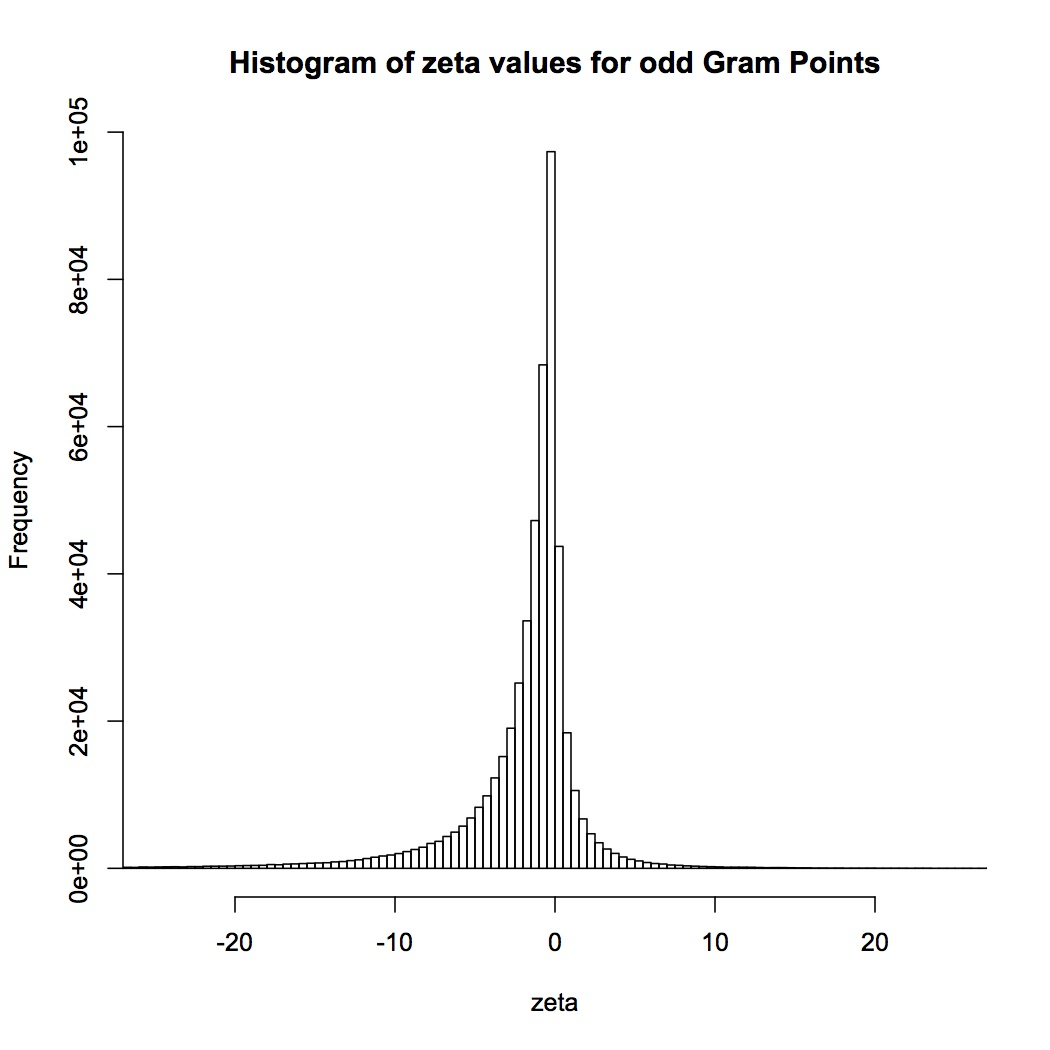
\includegraphics[width=0.62\textwidth]{ozeta.jpg}
\caption[]{ 
  Distribution of  $Z(t)$ at 500000 odd Gram points  at $t = 10^{12}$, i.e., $p_{odd}(y)$.
 }
\vspace{1mm}, 
\label{oddhist}

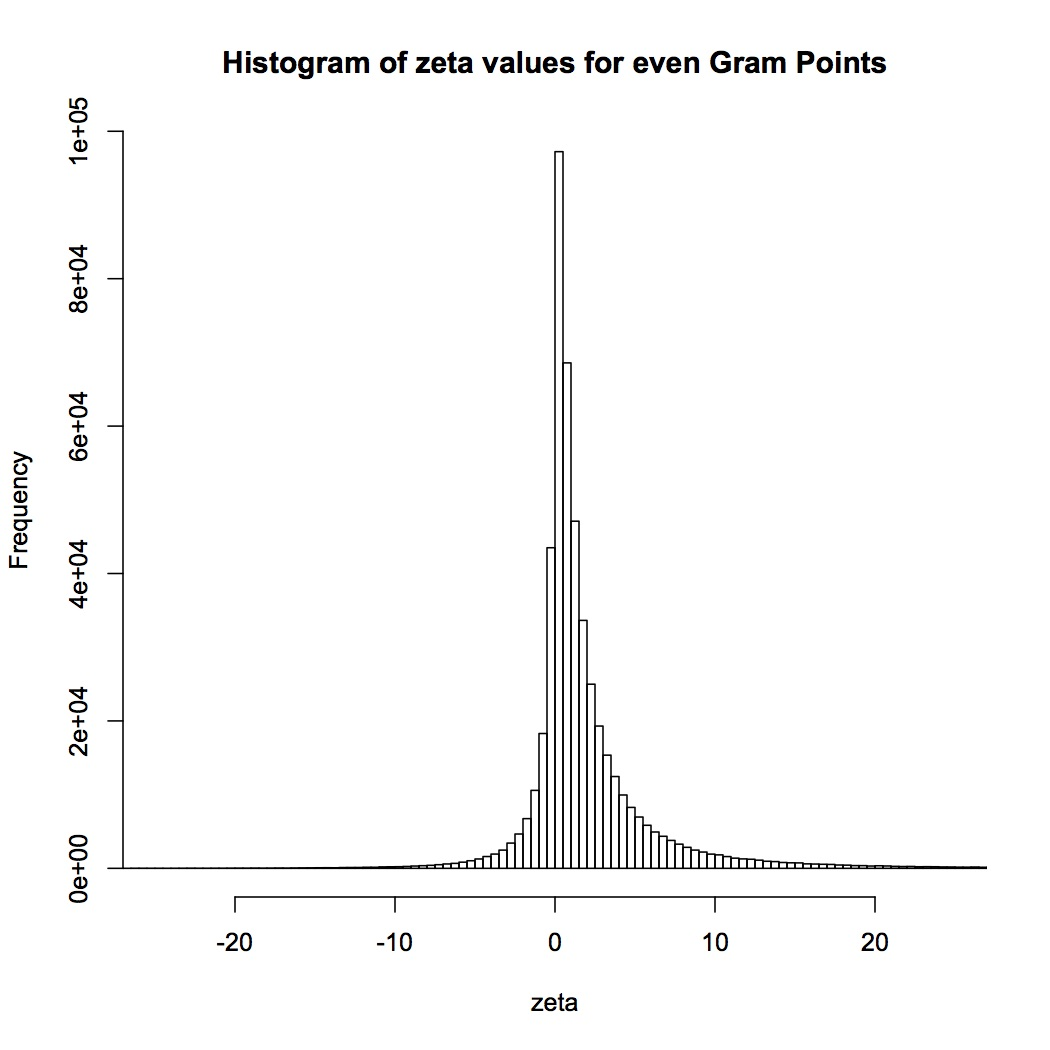
\includegraphics[width=0.62\textwidth]{ezeta.jpg}
\caption[]{ 
   Distribution of $Z(t)$ at 500000 even Gram points  at $t = 10^{12}$, i.e., $p_{even}(y)$.
 }
\label{evenhist}
\vspace{1mm}
\end{figure*}

\begin{table}
\centering \(\begin{array}{ccccccc}
\hline
 Gram &     Min.   & 1st    &  Median    &   Mean   & 3rd    &   Max. \\
 type &              & Quantile   &            &              & Quantile.    &   \\
\hline
All& -160.90 &   -1.17 &    0.00106 &   0.00  &  1.172 &165.10\\
Odd&-160.90 &   -2.526 &   -0.8471  & -2.00 &   -0.1121 &  69.41 \\
Even&-68.63 &   0.1139 &  0.8526  & 2.00 &   2.541 & 165.10 \\
\hline
\end{array}\)
\caption{Quantiles and mean for  $Z(t)$ at Gram points of different types.  The statistics are from $1$ million Gram intervals at $t=10^{12}$.} \label{tab:quantiles}
\end{table}


\begin{table}
\centering \(\begin{array}{ccccc}
\hline
 Gram~type&   --   & -+   & +-   & ++  \\
\hline
Odd & 0.151651&0.627465&0.069119&0.151765 \\
Even & 0.151565&0.069206&0.627551&0.151678 \\
\hline
\end{array}\)
\caption{Counts of different configurations of $Z(t)$  for pairs of consecutive Gram points.  The statistics are from $10$ million Gram intervals at $t=10^{15}$.} \label{tab:pairraw}
\end{table}

\begin{table}
\centering \(\begin{array}{ccccc}
\hline
 Gram~type&   --   & -+   & +-   & ++  \\
\hline
Odd & 0.151651&0.627465&0.069119&0.151765\\
\hline
Corresponding& 0.151678 & 0.627551 & 0.069206& 0.151565\\ 
Even~Entry     & (++)     & (+-)   & (-+)  & (--) \\
\hline
\end{array}\)
\caption{Test of Conjecture~\ref{antisymmetry} using pairs of consecutive Gram points.  The statistics are from $10$ million Gram intervals at $t=10^{15}$.} \label{tab:pairtest}
\end{table}


The empirical data presented in the  {previous sections led us to formulate the two conjectures stated in the introduction 
about the distribution of zeta values at the the Gram points. }
The evidence for  Conjecture~\ref{symmetry} has been presented in the previous sections. 
In this section we will consider the statistics of zeta values at pairs of consecutive Gram points. We will look at the evidence for Conjecture \ref{antisymmetry}.  

Table~\ref{tab:quantiles} shows the quantiles and mean for  $Z(t)$ at Gram points of different types.  The statistics are from $1$ million Gram intervals at $t=10^{12}$. They support 
Conjecture \ref{antisymmetry}., i.e.,  $p_{odd}(y) = p_{even}(-y)$.
Figures~\ref{oddhist} and \ref{evenhist}  present the histograms of $Z(t)$ at odd Gram points and even Gram points respectively. These figures further bear out the evidence of Table~\ref{tab:quantiles} that the odd and even distributions are mirror images of each other. \textcolor{blue}{ The distributions in Figures~\ref{oddhist} and \ref{evenhist} are clearly not symmetric, and hence they do not fit a normal distribution. We investigated whether the values could be distributed according to a beta distribution. Because of the large peaks in the distributions, the values of the beta distribution parameters had to be chosen to be quite large. Further investigation of the nature of the distribution needs to be done.
}

To study Conjecture \ref{antisymmetry} further, we will consider the zeta values at pairs of consecutive Gram points. We will classify the zeta values into two classes, '$+$' for positive $Z(t)$  ($Z(t) > 0$) and '$-$' for negative $Z(t)$ ($Z(t) \leqslant  0$). Thus, for example, the notation '$++$' stands for a Gram point which has a positive $Z(t)$ followed by a Gram point which has a positive $Z(t)$, while the notation '$+-$' stands for a Gram point which has a positive $Z(t)$ followed by a Gram point which has a negative $Z(t)$. Table~\ref{tab:pairraw} shows the counts for different pair configurations, for pairs beginning at odd Gram points (row 1) and for pairs beginning at even Gram points(row 2). Conjecture \ref{antisymmetry} predicts that the count for a configuration from the odd Gram point row in the table  will match the count for the mirror configuration in the even Gram point row of the table ( e.g., the count for '$++$' from the distribution for odd Gram points will match count for '$--$' from the distribution for even Gram points). Table~\ref{tab:pairtest} tests this prediction. The agreement is good, within the expected statistical variations. 

\section{\label{machineLearning}Machine Learning applications}

 { 
In this section we digress a bit and speculate on possible lessons of the present study for Machine Learning applications to the study of the Riemann zeta zeros \cite{osneural,osentropy}.
Why do we think that machine learning is a good tool to apply to the study of the zeros? It is because Machine Learning is an excellent tool to extract patterns when one has a huge amount of data and one does not have a complete understanding of the patterns underlying the phenomenon being studied. And indeed, with tens of trillions of the Riemann zeta function having been evaluated, one has the huge data set which would enable the application of machine learning techniques. Another encouraging indication that machine learning will be useful is a study of the entropy of the Riemann zeta zeros~\cite{osentropy}, which shows that the pattern of zeros shows a good amount of order.
}
\subsection{\label{secfeature}Neural Networks: feature selection}
 { 
How can we apply Machine Learning techniques to the problem? This is an open question, and one can think of different possible applications. Here we review a case study which used neural networks. A great deal of effort has gone into finding the zeros of the Riemann zeta function. At large heights finding the zeros is a non-trivial task, requiring much computer time (and some knowledge of special techniques to find the roots). It would be useful to have some guide to the location of the roots. In particular, close pairs of zeros are interesting. They correspond to cases for which the
Riemann Hypothesis is nearly false. Calculating the Riemann zeta function in zones where
two zeros are very close is a stringent test of the Riemann Hypothesis. Probably the biggest open task is to identify a feature set which is good at predicting zero differences, while not requiring excessive computing time. Ref~\cite{osneural} found that the behavior of the zeta function at Gram points is a good starting point to extract features for use in prediction. Our current study, indicating that Gram points have interesting properties which distinguish them from random points on the critical line, support the conclusion. The results of the present study suggest that it may be useful to extend the neural network application by separating the odd and even Gram points, and building separate models for them. Given the symmetry properties of the zeta values, we will probably find that the two models will be closely related to each other.  Furthermore, one can use symmetry properties of the zeta values at Gram points to impose restrictions on the models to be fitted.  
}

\subsection{\label{secMLrare}Machine Learning: detection of rare events}

 { 
We now discuss another possible approach to the solution. We have available to us extensive compilations of the location of zeros. The main challenge is that the phenomenon we are trying to detect, namely zeros which are located close to each other, is very rare. 
}

{ 
Ref~\cite{Friedman(2001)} suggest that  a good approach to detecting rare events is to estimate the expected probability density for the feature set, and to use the estimated probability density to identify values of the observed features which are anomalous, in that the estimated probability for the occurrence of the observed values is below a set threshold. The hope is that the places where the anomalous feature values occur are the places where the Riemann zeta zeros deviate from the normal pattern of behavior. The deviations could be of different types (small zero differences, large zero differences, etc.). If the classifier is sufficiently selective, then we will have a smaller number of roots that we have to evaluate to check for interesting behavior. 
}

{ 
Density estimation is a hard problem. Section 14.2.4 of \cite{Friedman(2001)}  discuss a technique for transforming the density estimation problem into one of supervised function approximation. To learn the input density, we generate two sets of data. The first set (class 0) contains the actual (sampled) inputs from the training data, whereas the second set (class 1) consists of randomly-generated feature values. Class 0 represents a sample representing the actual density function, and class 1 represents samples drawn from the same input space, with a uniform density function. Given this, the two data sets are then used to learn a logistic regression model, whose output can be interpreted as an approximate estimate of the actual density of the input. \textcolor{blue}{See~\cite{Friedman(2001)} for further discussion.}
          
}

\section{\label{conclusions}Conclusions}

In this work we presented a new  relation (Eq.~\ref{eq:consistency}) for the ratio of good to bad Gram points. We presented two conjectures regarding the distribution of zeta function values at Gram points. The conjectures refer to the even-odd Gram point antisymmetry Conjecture~\ref{antisymmetry}, and the forward-backward symmetry Conjecture~\ref{symmetry} (``time reversal" symmetry, if we think of the zeta values at Gram points as being a time series). After briefly describing the theory of the Riemann zeta function and the numerical evaluation, we presented statistics of the zeta function values. The statistics provide validation for the two conjectures.

Further study of the theoretical underpinnings of the observations in this work would likely give us a deeper insight into the properties of the Riemann zeta function. The symmetry properties could also aid us in choosing feature sets for Machine Learning applications to the study of the Riemann zeta zeros \cite{osneural,osentropy}.

\begin{thebibliography} {}

\bibitem{Sarnak 2005} Peter Sarnak,
``Problems of the Millennium: The Riemann Hypothesis (2004)",  {\it Clay Mathematics Institute Annual Report}, ( 2004), 
16-21

\bibitem{Gram 1903} J. P. Gram, 
``Sur les Zeros de la Fonction  $\zeta ( s )$  de Riemann",
{\it Acta Math.} {\bf27}(1903), 289-304

\bibitem{Odlyzko 1992}  A. Odlyzko,
``The $10^{20}$-th Zero of the Riemann Zeta
Function and 175 Million of its Neighbors", report,
\url{http://www.dtc.umn.edu/~odlyzko/unpublished/zeta.10to20.1992.pdf}, (1992)


\bibitem {Riemann(1858)} B. Riemann, ``\"{U}ber die Anzahl der Primzahlen uter
Einer Gegebenen Gr\"{o}be,'' {\it Montasb. der Berliner Akad.}, (1858),
671-680

\bibitem {Riemann 1892} B. Riemann, ``Gesammelte Werke'', Teubner, Leipzig, (1892)

\bibitem {Titchmarsh 1986} E. Titchmarsh, ``The Theory of the Riemann Zeta
Function,'' Oxford University Press, Second Edition, (1986)

\bibitem {Edwards(1974)} H. M. Edwards, ``Riemann's Zeta Function,''
Academic Press,  (1974)

\bibitem{os6} O. Shanker, 
``Generalised Zeta Functions and Self-Similarity of Zero Distributions",
{\it J.  Phys. A} {\bf39}(2006), 13983-13997

\bibitem {Matiyasevich} Y. Matiyasevich, 
``An artless method for calculating approximate values of
zeros of Riemann zeta function",
Web report, \url{http://logic.pdmi.ras.ru/~yumat/
personaljournal/artlessmethod/artlessmethodtexts.php}, (2013)

\bibitem{Hutchinson 1925} J. I. Hutchinson,
``On the roots of the Riemann zeta-function",
{\it Trans. Amer. Math.Soc.} {\bf27}(1925), 49-60

\bibitem{Korolev} M. A. Korolev,
``The Gram law and Selberg's conjecture on the distribution of zeros
of the Riemann zeta-function",
{\it Izv. Math.} {\bf74}:4(2010)

\bibitem{Titchmarsh 1935} E. C. Titchmarsh,
``The zeros of the Riemann zeta-function",
{\it Proc. Roy. Soc. London Ser. A} {\bf151}(1935), 234-255

\bibitem{Titchmarsh 1936} E. C. Titchmarsh,
``The zeros of the Riemann zeta-function",
{\it Proc. Roy. Soc. London Ser. A} {\bf157}(1936), 261-263

\bibitem{hiary} G. A. Hiary,
``Fast methods to compute the Riemann zeta function",
{\it Annals of Mathematics} {\bf174}(2011), 891-946

\bibitem{gourdon} Xavier Gourdon,
``The $10^{13}$ first zeros of the Riemann Zeta function,
and zeros computation at very large height", report,
\url{http://numbers.computation.free.fr/Constants/Miscellaneous/zetazeros1e13-1e24.pdf}, (2004)

\bibitem{hiary 2010} G. A. Hiary,
``An amortized-complexity method to compute the Riemann zeta function", 
\textcolor{blue}{{\it Mathematics of Computation} {\bf80}(2011), 1785-1796
}

\bibitem{osneural} O. Shanker, ``Neural Network prediction of Riemann zeta zeros''
{\it Advanced Modeling and Optimization}, {\bf 14}, 717-728, (2012). 

\bibitem{osentropy} O. Shanker, ``Entropy of Riemann zeta zero sequence''
{\it Advanced Modeling and Optimization}, {\bf 13}, 449-456, (2013). 

\bibitem {Friedman(2001)} J. Friedman, T. Hastie, and R. Tibshirani, ``The Elements of Statistical Learning,''
Springer,  (2001) 

\end{thebibliography} 

\end{document} 
